\documentclass[onecolumn]{revtex4}

\usepackage{graphicx}

\begin{document}

\title{
Final Project Write Up
}

\author{Mitchell Braun}

\affiliation{Siena College, Loudonville, NY}

\date {Today's date is November 30th, 2016}


\begin{abstract}

	Using the Monte Carlo method, I was able to calculate the odds that it would rain once and only one during each month while there was a 20 percent chance for rain on any given day. After creating a function that used the Monte Carlo approach, I was able to conclude that there was approximately a 0.9 percent chance that it would rain once and only once a month over a period of 100000 months. Also, after slightly adjusting my previous function, I was able to calculate the percentage that it would rain at least 8 days in a given month, while there was a 10 percent chance it would rain on any given day. For the same period of 100000 months, I concluded that there would be an approximately 0.8 percent chance that it would rain at least 8 days in a given month. 

\end{abstract}

\maketitle
 %%%%%%%%%%%%%%%%%%%%%%%%%%%%%%%%%%%%%%%%%%%%%%%%%%%%%%%%%%%%%%%%%%%%%

\section{Introduction}


	Throughtout this final project, I was tasked with the calculation of the odds of rainfall both analytically, by using a formula, and numerically by using the Monte Carlo Method of calculation. In order to complete this project, I made use of multiple functions, a few loops and a multitude of (if) statements with specific conditionals. Most importantly, I used the generation of random numbers extensively in order to create a significant number of senarios for which I would use to calculate the percentage or the amount of rain for any given month.

	

%%%%%%%%%%%%%%%%%%%%%%%%%%%%%%%%%%%%%%%%%%%%%%%%%%%%%%%%%%%%%%%%%%%%%

\section{Analytic Formula}

	This is the formula I used to analytically calculate the odds it would rain, where n equals the number of days it rained in a month.

	$$ Probability = 30 * (0.2)^n * (0.8)^{30 - n}$$

\section{Problem 1}

	In this problem, I was tasked with calculating the odds that it would rain once and only once in a given month, while there was a 20 percent chance it would rain on any given day. To answer this problem, I created a function that, when called, outputs the approximate percentage that it would rain once and only once during any given month. In this function I created 2 loops. First, I created a variable that was equal to the number of months I want to loop over, and established a counter that kept track of the months when it only rained once. I then looped over those months and established a counter that kept track of the days it rained in each month. Next, I created a loop that looped over 30 days and then generated a random number and checked to see if that number was between 0 and 0.2 and if it was, I added one to the counter which tracked the days it rained in each month. Then, I checked that when the counter which tracked these rainy days equaled one each time through the loop, I added 1 to the tracker that keeps track of the months where it rained once and only once. Finally, I divided the number of months when it only rained once and only once by the total number of months that I established in the beginning of the function.

%%%%%%%%%%%%%%%%%%%%%%%%%%%%%%%%%%%%%%%%%%%%%%%%%%%%%%%%%%%%%%%%%%%%%

\section{Problem 2}

	This problem was relatively simple after completing the previous problem because I had already created a function that calculated the odds it would rain once and only once in a giving month, so with some tweaking it would output the odds it would rain at least 8 times in a given month. In this problem, I was tasked with calculating the odds that it would rain at least 8 times in a given month, while there was a 10 percent chance it would rain on any given day. To answer this problem, I created a function that, when called, outputs the approximate percentage that it would rain once and only once during any given month. In this function I created 2 loops. First, I created a variable that was equal to the number of months I want to loop over, and established a counter that kept track of the months when it only rained once. I then looped over those months and established a counter that kept track of the days it rained in each month. Next, I created a loop that looped over 30 days and then generated a random number and checked to see if that number was between 0 and 0.1 and if it was, I added one to the counter which tracked the days it rained in each month. Then, I checked that when the counter which tracked these rainy days was greater than or equal to 8 each time through the loop, I added 1 to the tracker that keeps track of the months where it rained at least 8 times in a given month. Finally, I divided the number of months when it rained at least 8 times in a given month by the total number of months that I established in the beginning of the function.

%%%%%%%%%%%%%%%%%%%%%%%%%%%%%%%%%%%%%%%%%%%%%%%%%%%%%%%%%%%%%%%%%%%%%

\section{Problem 3A}

	Unfortunately, I was unable to fully complete this problem. However, I was able to create a function that was able to return the amount of rainfall during a given month. To do this, my function looped over 30 days and generated a random number between 0 and 1. I then checked this random number to see if it met the conditionals outlined in the problem. In order to visualize the conditionals, I used the idea of  a number line ranging from 0 to 1. For example, if  the random number was in between 0 and 0.2 on the number line, then there was a 20 percent chance that it would rain 1 cm. However, to account for the fact that both 2 and 3 cm had a 30 percent chance to occur, I added 0.3 to 0.2 from the previous conditional which brought me to 0.5 on the number line. Now, this range between 0.2 and 0.5 represents 2 cm. I then added 0.3 to the 0.5 conditional, resulting in the range of 0.5 to 0.8 which represents 3 cm. Additionally, I did this same approach for the 4 and 5 cm parameters, however I added 0.1 to each conditional rather than 0.3. The second function present is incomplete, however I attempted to loop over 1000 months and use a list in order to complete each parameter. However, I was unsuccessful.

%%%%%%%%%%%%%%%%%%%%%%%%%%%%%%%%%%%%%%%%%%%%%%%%%%%%%%%%%%%%%%%%%%%%%

\section{Problem 3B}

\begin{figure}[h]

	\centering
	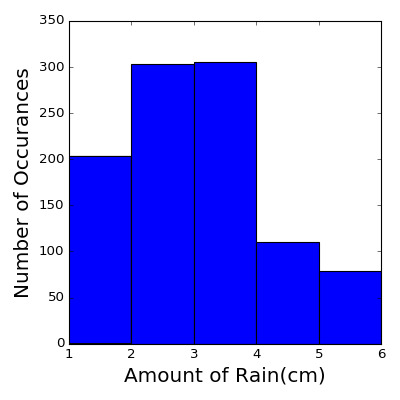
\includegraphics[width=0.4\textwidth]{Final_Histogram.png}
	\caption{This is my histogram created using the results of my first function in 3A.}


\end{figure}

\subsection{Histogram}

	To create this histogram, I looped over 1000 months and appended the results of my first function 3A, which calculated the amount of rainfall, for those 1000 months to a list. Then, I ploted the list using 5 bins in order display the complete set of data accurately. Finally, I adjusted the layout in order to achieve the perfect orientation for the histogram.

%%%%%%%%%%%%%%%%%%%%%%%%%%%%%%%%%%%%%%%%%%%%%%%%%%%%%%%%%%%%%%%%%%%%%

\section{Conclusion}

	To me, this final project was extremely beneficial because it definitely broaded my knowledge on both the Monte Carlo Method of calculation and the use of functions, loops and "if" statements in order to estimate probability. This project was challenging, however once I figured out each problem, I was overwhelmed with satisfaction because of the hard work and time I put into it. In conclusion, I believe that this final project definitely helped me learn more about the implication of the Monte Carlo Method of calculation in order to solve a wide range of problems.

	

\end{document}


